\chapter{Lukuteoria}

Lukuteoria on kokonaislukuja tutkiva matematiikan ala,
jonka keskeinen teema on lukujen jaollisuus.
Tyypillinen lukuteorian tehtävä on selvittää,
onko luku alkuluku tai mitkä ovat sen alkutekijät.
Tässä luvussa tutustumme kisakoodauksessa usein
tarvittaviin lukuteorian algoritmeihin.

\section{Jaollisuus ja alkuluvut}

Luku $a$ on luvun $b$ jakaja eli tekijä,
jos $b$ on jaollinen $a$:lla.
Jos $a$ on $b$:n jakaja,
niin merkitään $a \mid b$,
ja muuten merkitään $a \nmid b$.
Esimerkiksi luvun 24 jakajat ovat 1, 2, 3, 4, 6, 8, 12 ja 24.

Luku $n$ on alkuluku, jos sen ainoat jakajat ovat 1 ja $n$.
Esimerkiksi luvut 7, 19 ja 41 ovat alkulukuja.
Luku 35 taas ei ole alkuluku, koska $5 \cdot 7 = 35$.
Jokaiselle luvulle $n>1$ on olemassa yksikäsitteinen
alkutekijähajotelma
\[ n = p_1^{a_1} p_2^{a_2} \cdots p_k^{a_k},\]
jossa $p_1,p_2,\ldots,p_k$ ovat alkulukuja.
Alkutekijähajotelman avulla saa laskettua
luvun $n$ jakajien määrän kaavalla,
\[m(n)=\prod_{i=1}^k (a_i+1)\]
jakajien summan kaavalla
\[s(n)=\prod_{i=1}^k \frac{p_i^{a_i+1}-1}{p_i-1}.\]
sekä jakajien tulon kaavalla
\[t(n)=n^{m(n)/2}.\]

Esimerkiksi luvun $1176$ alkutekijähajotelma on
$2^3 \cdot 3^1 \cdot 7^2$,
jakajien määrä on $(3+1)(1+1)(2+1)=24$,
summa on $\frac{2^4-1}{2-1} \cdot \frac{3^2-1}{3-1} \cdot \frac{7^3-1}{7-1} = 3420$
ja tulo on $1176^{12}$.

\subsection{Perusalgoritmit}

Jos luku $n$ ei ole alkuluku,
niin sen voi esittää muodossa $a \cdot b$,
missä $a \le \sqrt n$ tai $b \le \sqrt n$,
minkä ansiosta sillä on varmasti
tekijä välillä $2 \ldots \sqrt n$.
Tämän havainnon avulla voi tarkastaa ajassa $O(\sqrt n)$,
onko luku alkuluku vai ei,
sekä myös selvittää ajassa $O(\sqrt n)$
luvun alkutekijähajotelman.

Seuraava funktio \texttt{prime} selvittää,
onko annettu luku $n$ alkuluku.
Funktio koettaa jakaa lukua kaikilla luvuilla
välillä $2 \ldots \sqrt n$, ja jos mikään
luvuista ei jaa $n$:ää, niin $n$ on alkuluku.

\begin{lstlisting}
bool prime(int n) {
    if (n < 2) return false;
    for (int x = 2; x*x <= n; x++) {
        if (n%x == 0) return false;
    }
    return true;
}
\end{lstlisting}

\noindent
Seuraava funktio \texttt{factors} muodostaa
vektorin, joka sisältää luvun $n$
alkutekijähajotelman.
Funktio jakaa $n$:ää sen alkutekijöillä ja lisää
niitä samaan aikaan vektoriin.
Prosessi päättyy, kun jäljellä on luku $n$,
jolla ei ole tekijää välillä $2 \ldots \sqrt n$.
Jos $n>1$, se on alkuluku ja viimeinen tekijä.

\begin{lstlisting}
vector<int> factors(int n) {
    vector<int> f;
    for (int x = 2; x*x <= n; x++) {
        while (n%x == 0) {
            f.push_back(x);
            n /= x;
        }
    }
    if (n > 1) f.push_back(n);
    return f;
}
\end{lstlisting}

Huomaa, että funktio lisää jokaisen alkutekijän
niin monta kertaa, kuin se jakaa luvun.
Esimerkiksi $24=2^3 \cdot 3$,
joten funktio tuottaa vektorin $[2,2,2,3]$.

\subsection{Eratostheneen seula}

Eratostheneen seula on esilaskenta-algoritmi,
jonka suorituksen jälkeen mistä tahansa
välin $2 \ldots n$ luvusta pystyy tarkastamaan
tehokkaasti, onko se alkuluku,
sekä etsimään yhden luvun alkutekijän,
jos luku ei ole alkuluku.

Algoritmi luo taulukon $\texttt{a}$,
jossa $\texttt{a}[k]=0$ tarkoittaa,
että $k$ on alkuluku,
ja $\texttt{a}[k] \neq 0$ tarkoittaa,
että $k$ ei ole alkuluku.
Jälkimmäisessä tapauksessa $\texttt{a}[k]$
on yksi $k$:n alkutekijöistä.

Eratostheneen seula käy läpi välin
$2 \ldots n$ lukuja yksi kerrallaan.
Aina kun uusi alkuluku $x$ löytyy,
niin algoritmi merkitsee taulukkoon, että $x$:n moninkerrat
$2x,3x,4x,\ldots$ eivät ole alkulukuja,
koska niillä on alkutekijä $x$.

\noindent
Esimerkiksi jos väli on $2 \ldots 20$,
taulukosta tulee:

\begin{center}
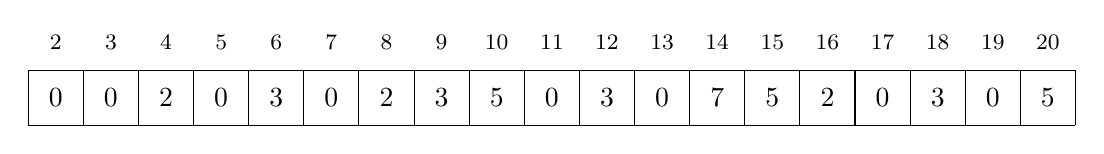
\begin{tikzpicture}[scale=0.7]
\draw (0,0) grid (19,1);

\node at (0.5,0.5) {$0$};
\node at (1.5,0.5) {$0$};
\node at (2.5,0.5) {$2$};
\node at (3.5,0.5) {$0$};
\node at (4.5,0.5) {$3$};
\node at (5.5,0.5) {$0$};
\node at (6.5,0.5) {$2$};
\node at (7.5,0.5) {$3$};
\node at (8.5,0.5) {$5$};
\node at (9.5,0.5) {$0$};
\node at (10.5,0.5) {$3$};
\node at (11.5,0.5) {$0$};
\node at (12.5,0.5) {$7$};
\node at (13.5,0.5) {$5$};
\node at (14.5,0.5) {$2$};
\node at (15.5,0.5) {$0$};
\node at (16.5,0.5) {$3$};
\node at (17.5,0.5) {$0$};
\node at (18.5,0.5) {$5$};

\footnotesize

\node at (0.5,1.5) {$2$};
\node at (1.5,1.5) {$3$};
\node at (2.5,1.5) {$4$};
\node at (3.5,1.5) {$5$};
\node at (4.5,1.5) {$6$};
\node at (5.5,1.5) {$7$};
\node at (6.5,1.5) {$8$};
\node at (7.5,1.5) {$9$};
\node at (8.5,1.5) {$10$};
\node at (9.5,1.5) {$11$};
\node at (10.5,1.5) {$12$};
\node at (11.5,1.5) {$13$};
\node at (12.5,1.5) {$14$};
\node at (13.5,1.5) {$15$};
\node at (14.5,1.5) {$16$};
\node at (15.5,1.5) {$17$};
\node at (16.5,1.5) {$18$};
\node at (17.5,1.5) {$19$};
\node at (18.5,1.5) {$20$};

\end{tikzpicture}
\end{center}

\noindent
Seuraava koodi toteuttaa
Eratostheneen seulan.
Koodi olettaa, että jokainen taulukon \texttt{a}
alkio on aluksi 0.

\begin{lstlisting}
for (int x = 2; x <= n; x++) {
    if (a[x]) continue;
    for (int u = 2*x; u <= n; u += x) {
        a[u] = x;
    }
}
\end{lstlisting}

\noindent
Algoritmin sisäsilmukka suoritetaan
$n/i$ kertaa tietyllä $i$:n arvolla,
joten algoritmin ajankäyttöä arvioi harmoninen summa
$\sum_{i=2}^n n/i = n/2 + n/3 + n/4 + \cdots + n/n$.
Harmonisen summan suuruus on luokkaa $O(n \log n)$,
mikä on yläraja algoritmin ajankäytölle.
Todellisuudessa Eratostheneen seula on vielä nopeampi,
koska sisäsilmukka suoritetaan vain,
jos luku on alkuluku.

\subsection{Eukleideen algoritmi}

Lukujen $a$ ja $b$ suurin yhteinen tekijä eli $\textrm{syt}(a,b)$
on suurin luku, jolla sekä $a$ että $b$ on jaollinen.
Esimerkiksi $\textrm{syt}(30,42)=6$.
Vastaavasti pienin yhteinen moninkerta eli $\textrm{pym}(a,b)$
on pienin luku, joka on jaollinen sekä $a$:lla että $b$:llä.
Näiden lukujen välillä on yhteys $\textrm{pym}(a,b)=ab/\textrm{syt}(a,b)$.

Eukleideen algoritmi on tehokas tapa etsiä
lukujen $a$ ja $b$ suurin yhteinen tekijä $\textrm{syt}(a,b)$.
Se laskee suurimman yhteisen tekijän kaavalla
\begin{equation*}
    \textrm{syt}(a,b) = \begin{cases}
               a        & b = 0\\
               \textrm{syt}(b,a \bmod b) & b \neq 0\\
           \end{cases}
\end{equation*}

\noindent
Esimerkiksi $\textrm{syt}(24,36) = \textrm{syt}(36,24)
= \textrm{syt}(24,12) = \textrm{syt}(12,0)=12$.
Eukleideen algoritmi on tehokas
algoritmi, ja on mahdollista osoittaa,
että sen aikavaativuus on vain $O(\log n)$,
kun $n=\min(a,b)$.

\subsection{Eulerin totienttifunktio}

Luvut $a$ ja $b$ ovat suhteelliset alkuluvut,
jos $\textrm{syt}(a,b)=1$.
Eulerin totienttifunktio $\varphi(n)$
laskee luvun $n$ suhteellisten alkulukujen
määrän välillä $1 \ldots n$.
Esimerkiksi $\varphi(12)=4$,
koska 1, 5, 7 ja 11 ovat suhteellisia
alkulukuja 12:n kanssa.

Totienttifunktion arvon $\varphi(n)$ pystyy laskemaan
luvun $n$ alkutekijähajotelmasta kaavalla
\[ \varphi(n) = \prod_{i=1}^k p_i^{a_i-1}(p_i-1). \]
Esimerkiksi $\varphi(12)=2^1 \cdot (2-1) \cdot 3^0 \cdot (3-1)=4$.
Huomaa myös, että $\varphi(n)=n-1$,
jos $n$ on alkuluku.

\section{Modulolaskenta}

Modulolaskennan peruslaskusäännöt ovat:

\[
\begin{array}{lcl}
(x+y) \bmod M & = & (x \bmod M + y \bmod M) \bmod M \\
(x-y) \bmod M & = & (x \bmod M - y \bmod M) \bmod M \\
(x \cdot y) \bmod M & = & (x \bmod M \cdot y \bmod M) \bmod M \\
(x^k) \bmod M & = & (x \bmod M)^k \bmod M \\
\end{array}
\]

\subsection{Tehokas potenssilasku}

Modulolaskennassa tulee usein tarvetta laskea
tehokkaasti potenssilasku $x^n$.
Tämä onnistuu ajassa $O(\log n)$
seuraavan rekursion avulla:
\begin{equation*}
    x^n = \begin{cases}
               1        & n = 0\\
               x^{n/2} \cdot x^{n/2} & \text{$n$ on parillinen}\\
               x^{n-1} \cdot x & \text{$n$ on pariton}
           \end{cases}
\end{equation*}

Oleellista on, että parillisen $n$:n
tapauksessa luku $x^{n/2}$ lasketaan vain kerran.
Tämän ansiosta potenssilaskun aikavaativuus on $O(\log n)$,
koska $n$:n koko puolittuu aina silloin,
kun $n$ on parillinen.

\subsection{Eulerin lause}

Eulerin lauseen mukaan
\[x^{\varphi(M)} \bmod M = 1,\]
kun $x$ ja $M$ ovat suhteelliset alkuluvut.
Kun $M$ on alkuluku, saadaan lause
\[x^{M-1} \bmod M = 1,\]
jonka seurauksena
\[(x^k) \bmod M =  (x^{k \bmod (M-1)}) \bmod M,\]
kun $x$ ja $M$ ovat suhteelliset alkuluvut.

\subsection{Modulon käänteisluku}

Luvun $x$ käänteisluku modulo $M$
tarkoittaa sellaista lukua $x^{-1}$,
että
\[ x x^{-1} \bmod M = 1. \]
Esimerkiksi jos $x=6$ ja $M=17$,
niin $x^{-1}=3$, koska $(6\cdot3) \bmod 17=1$.

Modulon käänteisluku mahdollistaa
jakolaskun laskemisen modulossa
olevilla luvuilla,
koska jakolasku luvulla $x$ vastaa
kertolaskua luvulla $x^{-1}$.
Esimerkiksi lasku $36/6=6$ laskettuna
modulo 17 on $2 \cdot 3 = 6$.

Toisin kuin tavallinen jakolasku,
modulon jakolasku ei ole aina mahdollista suorittaa.
Käänteisluku $x^{-1}$ modulossa $M$
on olemassa vain silloin,
kun $x$ ja $M$ ovat suhteellisia alkulukuja.

Modulon käänteisluvun saa laskettua kaavalla
\[
x^{-1} = x^{\varphi(M)-1}.
\]

Jos $M$ on alkuluku, kaavasta tulee
\[
x^{-1} = x^{M-2}.
\]

Esimerkiksi jos $x=6$ ja $M=17$, niin
$x^{-1}=6^{17-2} \bmod 17 = 3$.

Modulon käänteisluvun kaava perustuu Eulerin
lauseeseen.
Modulon käänteisluvulle täytyy päteä
\[
x x^{-1} \bmod M = 1.
\]
Toisaalta Eulerin kaavan perusteella
\[
xx^{\varphi(M)-1} \bmod M = 1,
\]
eli lukujen $x^{-1}$ ja $x^{\varphi(M)-1}$ on oltava samat.

\section{Yhtälönratkaisu}

\subsection{Diofantoksen yhtälö}

Diofantoksen yhtälö on muotoa
\[ ax + by = c, \]
missä $a$, $b$ ja $c$ ovat vakioita
ja tehtävänä on ratkaista muuttujat $x$ ja $y$.
Kaikki luvut yhtälössä ovat kokonaislukuja.
Esimerkiksi jos yhtälö on $5x+2y=11$, yksi ratkaisu
on valita $x=3$ ja $y=-2$.

Diofantoksen yhtälön voi ratkaista
tehokkaasti Eukleideen algoritmin avulla,
koska Eukleideen algoritmia laajentamalla
pystyy löytämään luvun $\textrm{syt}(a,b)$
lisäksi luvut $x$ ja $y$,
jotka toteuttavat yhtälön
\[
ax + by = \textrm{syt}(a,b) \cdot z.
\]
Alkuperäisen yhtälön ratkaisu on olemassa, jos $c$ on
jaollinen $\textrm{syt}(a,b)$:llä,
ja muussa tapauksessa yhtälöllä ei ole ratkaisua.

\subsubsection*{Laajennettu Eukleideen algoritmi}

Etsitään esimerkkinä luvut $x$ ja $y$,
jotka toteuttavat yhtälön
\[
39x + 15y = 12,
\]
Yhtälöllä on ratkaisu, koska $\textrm{syt}(39,15)=3$
ja $3 \mid 12$.
Kun Eukleideen algoritmi laskee lukujen
39 ja 15 suurimman
yhteisen tekijän, syntyy ketju
\[
\textrm{syt}(39,15) = \textrm{syt}(15,9)
= \textrm{syt}(9,6) = \textrm{syt}(6,3)
= \textrm{syt}(3,0) = 3. \]
Algoritmin aikana muodostuvat jakoyhtälöt ovat:
\[
\begin{array}{lcl}
39 - 2 \cdot 15 & = & 9 \\
15 - 1 \cdot 9 & = & 6 \\
9 - 1 \cdot 6 & = & 3 \\
\end{array}
\]
Näiden yhtälöiden avulla saadaan
\[
39 \cdot 2 + 15 \cdot (-5) = 3
\]
ja kertomalla yhtälö 4:lla tuloksena on
\[
39 \cdot 8 + 15 \cdot (-20) = 12,
\]
joten alkuperäisen yhtälön ratkaisu on $x=8$ ja $y=-20$.

Diofantoksen yhtälön ratkaisu ei ole yksikäsitteinen,
vaan yhdestä ratkaisusta on mahdollista muodostaa
äärettömästi muita ratkaisuja.
Kun yhtälön ratkaisu on $(x,y)$,
niin myös $(x+k b/s,y-k a/s)$ on ratkaisu,
missä $s=\textrm{syt}(a,b)$ ja $k$
on mikä tahansa kokonaisluku.

\subsection{Kiinalainen jäännöslause}

Kiinalainen jäännöslause ratkaisee yhtälöryhmän muotoa
\[
\begin{array}{lcl}
x & = & a_1 \bmod M_1 \\
x & = & a_2 \bmod M_2 \\
\cdots \\
x & = & a_n \bmod M_n \\
\end{array}
\]
missä kaikki parit luvuista $M_1,M_2,\ldots,M_n$
ovat suhteellisia alkulukuja.

Olkoon $x^{-1}_M$ luvun $x$ käänteisluku
modulo $M$ ja

\[ X_k = \frac{M_1 M_2 \cdots M_n}{M_k}.\]

Näitä merkintöjä käyttäen yhtälöryhmän ratkaisu on
\[x = a_1 X_1 {X_1}^{-1}_{M_1} + a_2 X_2 {X_2}^{-1}_{M_2} + \cdots + a_n X_n {X_n}^{-1}_{M_n}.\]

Ideana on, että jokaisessa yhtälön osassa
$a_k X_k {X_k}^{-1}_{M_k}$
jakojäännös $M_k$:lla on $a_k$,
koska $X_k$ ja sen käänteisluku kumoavat toisensa.
Samaan aikaan kaikki muut yhtälön osat ovat jaollisia luvulla
$M_k$, eli ne eivät vaikuta jakojäännökseen ja
koko summan jakojäännös $M_k$:lla on $a_k$.

Esimerkiksi yhtälöryhmän
\[
\begin{array}{lcl}
x & = & 3 \bmod 5 \\
x & = & 4 \bmod 7 \\
x & = & 2 \bmod 3 \\
\end{array}
\]
ratkaisu on
\[ 3 \cdot 21 \cdot 1 + 4 \cdot 15 \cdot 1 + 2 \cdot 35 \cdot 2 = 263.\]

Kun luku $x$ on yhtälöryhmän ratkaisu,
niin myös kaikki luvut muotoa
$x+M_1 M_2 \cdots M_n$ ovat ratkaisuja.

